% 
% (c) Copyright 2016 Tabea Mendez
% 
% This source is free: you can redistribute it and/or modify
% it under the terms of the GNU General Public License as published by
% the Free Software Foundation, either version 3 of the License, or
% (at your option) any later version.
% 
% This source is distributed in the hope that it will be useful,
% but WITHOUT ANY WARRANTY; without even the implied warranty of
% MERCHANTABILITY or FITNESS FOR A PARTICULAR PURPOSE.  See the
% GNU General Public License for more details.
% 
% You should have received a copy of the GNU General Public License
% along with this source.  If not, see <http://www.gnu.org/licenses/>.
%
%%%%%%%%%%%%%%%%%%%%%%%%%%%%%%%%%%%%%%%%%%%%%%%%%%%%%%%%%%%%%%%%%%%%%%%%%%%%%%

Das Ziel ist mit einem Filter $H(z)$ bzw. dessen Impulsantwort $h(n)$ eine gewünschte Waveform zu generieren. Dazu gibt es zwei Möglichkeiten:
\begin{itemize}
 \item Die Waveform Sample für Sample berechnen (Impulsantwort $h(n)$ des Filters $H(z)$)
 \item Waveform vorab berechnen und in einer Wavetable abspeichern. Die Frequenz periodischer Signale kann so über die Auslesegeschwindigkeit gesteuert werden
\end{itemize}

\section{Sinus-Generator}
	\begin{tabular}{|c|c|}
	\hline&\\[-0.3cm]
		\textbf{Sinus-Signal-Generator} & \textbf{Cosinus-Signal-Generator}\\[0.1cm]
	\hline&\\[-0.2cm]
		\fcolorbox{CadetRed}{white}{$h(n) = R^n\,\sin(\omega_0n)\,u(n)$} & \fcolorbox{CadetRed}{white}{$h(n) = R^n\,\cos(\omega_0n)\,u(n)$}\\[0.4cm]
		\fcolorbox{CadetRed}{white}{$H(z) = \dfrac{R\,\sin(\omega_0)\,z^{-1}}{1-2\,R\,\cos(\omega_0)\,z^{-1}+R^2\,z^{-2}}$} & \fcolorbox{CadetRed}{white}{$H(z) = \dfrac{1 - R\,\cos(\omega_0)\,z^{-1}}{1-2\,R\,\cos(\omega_0)\,z^{-1}+R^2\,z^{-2}}$}\\[0.5cm]
		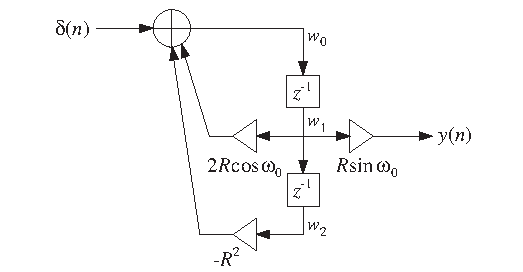
\includegraphics[width = 0.45\textwidth]{pic/sinusGen.pdf} & 
		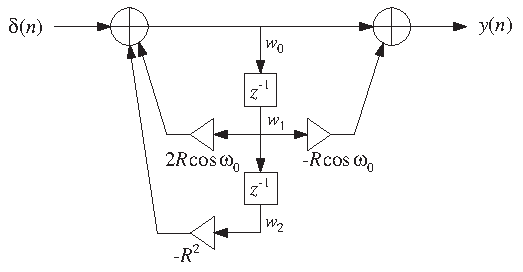
\includegraphics[width = 0.45\textwidth]{pic/cosinusGen.pdf}\\ 
		\fcolorbox{black}{white}{$\begin{array}{l}for\,\, n = 0,1,2,...\,\, do:\\
		\quad w_0 = 2R\cos(\omega_0)\,w_1 - R^2\,w_2 + \delta(n) \\
		\quad y = R\sin(\omega_0)\,w_1\\
		\quad w_2 = w_1\\
		\quad w_1 = w_0\end{array}$}& 
		\fcolorbox{black}{white}{$\begin{array}{l}for\,\, n = 0,1,2,...\,\, do:\\
		\quad w_0 = 2R\cos(\omega_0)\,w_1 - R^2\,w_2 + \delta(n) \\
		\quad y = w_0 - R\cos(\omega_0)\,w_1\\
		\quad w_2 = w_1\\
		\quad w_1 = w_0\end{array}$}\\[1.6cm]
	\hline\multicolumn{2}{|c|}{}\\[-0.3cm]
		\multicolumn{2}{|c|}{\textbf{Gekoppelter-Sinus-Cosinus-Generator}}\\[0.1cm]
	\hline\multicolumn{2}{|c|}{}\\[-0.2cm]
		\multicolumn{2}{|c|}{\fcolorbox{CadetRed}{white}{$h_1(n) = R^n\,\cos(\omega_0n)\,u(n)$}$\qquad$ \fcolorbox{CadetRed}{white}{$h_2(n) = R^n\,\sin(\omega_0n)\,u(n)$}}\\[0.35cm]
		\multicolumn{2}{|c|}{\fcolorbox{CadetRed}{white}{$H_1(z) = \dfrac{1 - a\,z^{-1}}{1-2\,a\,z^{-1}+(a^2+b^2)\,z^{-2}}$} $\qquad$ \fcolorbox{CadetRed}{white}{$H_2(z) = \dfrac{b\,z^{-1}}{1-2\,a\,z^{-1}+(a^2+b^2)\,z^{-2}}$}}\\[0.6cm]
		\multicolumn{2}{|c|}{\fcolorbox{CadetRed}{white}{$a = R\,\cos(\omega_0)$} $\qquad$ \fcolorbox{CadetRed}{white}{$b=R\,\sin(\omega_0)$}}\\[0.25cm]
		\multicolumn{2}{|c|}{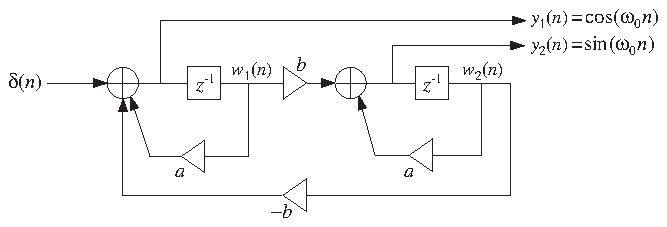
\includegraphics[width = 0.6\textwidth]{pic/sinusCosinusGen.pdf}}\\
		\multicolumn{2}{|c|}{\fcolorbox{black}{white}{$\begin{array}{l}for\,\, n = 0,1,2,...\,\, do:\\
		\quad y_1 = a\,w_1 - b\,w_2 + \delta(n) \\
		\quad y_2 = a\,w_2 + b\,w_1 \\
		\quad w_1 = y_1\\
		\quad w_2 = y_2\end{array}$}}\\[1.4cm]
	\hline
	\end{tabular}

\section{Periodische Waveform Generatoren}
	\subsection{Periodische Signale}
		\vspace*{-1.3cm}\begin{minipage}{0.6\textwidth}
			\begin{danger}
				Die abgetastete Version $x(n)$ eines periodischen Signals $x(t)$ ist nicht zwingend periodisch! 
			\end{danger}
		\end{minipage}\begin{minipage}{0.03\textwidth}$ $\end{minipage}
		\begin{minipage}{0.4\textwidth}
			\begin{tikzpicture}[>=latex', scale=3.3]
				\def\f{0.15};
				\draw[line width=0.5,->](-0.2,0)--++(2,0)node[right]{\small$t$};
				\draw[line width=0.5,->](0,-0.5)--++(0,1)node[right]{\small$x(t)$};
				\draw[smooth,samples=100,domain=0:1.7, CadetRed, line width=1] plot (\x,{0.35*sin(8*\x*180/pi)});
				\draw[smooth,samples=100,domain=-0.2:0, CadetRed, line width=1] plot (\x,{0});
				\foreach \i in {0,1,...,11}
				{
					\coordinate (sample) at ({\i*\f},{0.35*sin(8*\i*\f*180/pi)});
					\fill (sample) circle (0.65pt);
					\draw[line width=0.75](sample)--({\i*\f},0);
				}
				\draw[line width=0.5](0.787,0.05)--(0.787,-0.5);
				\draw[line width=0.5,<->](0,-0.43)--node[below]{\small$T_D$}++(0.787,0);

				\draw[line width=0.5](\f*3,0)--++(0,0.25);
				\draw[line width=0.5](\f*4,0)--++(0,0.25);
				\draw[line width=0.5,<->](\f*3,0.21)--node[above]{\small$T$}++(\f,0);

			\end{tikzpicture}
		\end{minipage}$ $\\[-1cm]
		Damit das abgetastete Signal $x(n)$ periodisch ist muss gelten:\\[0.15cm]
		\begin{tabular}{ll}
		 $\begin{array}{l}\text{$T_D$ ist ein ganzzahliges Vielfaches }\\\text{der Abtastperiode $T$}\end{array}$ & \fcolorbox{CadetRed}{white}{$T_D = D\cdot T$}$\quad\;\Rightarrow\quad\;$\fcolorbox{CadetRed}{white}{$f = \dfrac{f_s}{D}$}\\[0.5cm]
		 $\;\,$analoge Periodizität: & \fcolorbox{black}{white}{$x(t) = x(t + T_D)$}\\[0.2cm]
		 $\;\,$digitale Periodizität: & \fcolorbox{black}{white}{$x(nT) = x(nT + DT)  = x(nT + T_D)$}\\
		\end{tabular}\\
		
	\subsection{Realisierungsformen periodischer Waveform Generatoren}
		\begin{itemize}
		 \item Die ersten $D$-Samples ($h(0),...,h(D-1)$) mit einem FIR-Filter spezifizieren und das FIR-Filter periodisch mit Impulsen anregen ($\delta(n),\delta(n-D),\delta(n-2D),...$).
		 \item FIR-Filter $N(z)$:$\qquad\qquad\qquad\,$
		 \fcolorbox{CadetRed}{white}{$N(z) = b_0+b_1\,z^{-1}+b_2\,z^{-2}+...+b_{D-1}\,z^{-(D-1)}$}
		 \item Periodische Anregung $P(z)$:$\;\;\;\;\,$
		 \fcolorbox{CadetRed}{white}{$P(z) = 1 + z^{-D} + z^{-2D} + z^{-3D}+ ... = \dfrac{1}{1-z^{-D}}$}
		 \item Übertragungsfunktion $H(z)$:$\quad$
		 \fcolorbox{CadetRed}{white}{$H(z) = P(z)\cdot N(z) = \dfrac{b_0+b_1\,z^{-1}+b_2\,z^{-2}+...+b_{D-1}\,z^{-(D-1)}}{1-z^{-D}}$}
		 \item Impulsantwort $h(n)$:$\qquad\qquad\;\;\,$
		 \fcolorbox{CadetRed}{white}{$h(n) = \underbrace{h(n-D)}_{\text{weitere Perioden}} + \underbrace{b_0\,\delta(n)+b_1\,\delta(n-1)+...+b_{D-1}\,\delta(n-(D-1))}_{\text{1. Periode}}$}\\[0.2cm]
		 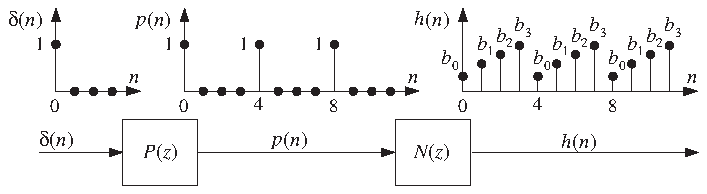
\includegraphics[width = 0.8\textwidth]{pic/periodischesDigitalesSignal.pdf}\\[-0.3cm]
		\end{itemize}
		
		\begin{minipage}{0.485\textwidth}
		\textbf{\textcolor{black}{\large{Implementierung mit Direktform}}}\\[-0.2cm]
			\begin{itemize}
			 \item Zustände $v_i$ und $w_i$ werden mit Null initialisiert.\\[-0.4cm]
			 \item FIR-Filter-Teil der angeregt wird, wodurch die ersten $D$ Samples generiert werden.\\[-0.4cm]
			 \item IIR-Filter-Teil der die $D$ Samples wiederholt.\\[-0.2cm]
			\end{itemize}
			\hspace*{0.3cm}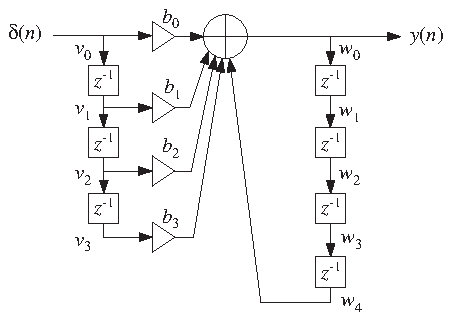
\includegraphics[width = 0.9\textwidth]{pic/periodischesWFGenDirektform.pdf}
		\end{minipage}\begin{minipage}{0.03\textwidth}$ $\end{minipage}
		\begin{minipage}{0.485\textwidth}
			\begin{tabular}{|lclll|}
			\hline &&&&$ $\\[-0.3cm]
			\multicolumn{5}{|l|}{$for\,\, n = 0,1,2,...\,\, do:$}\\
			&$v_0$&$ =$& $\delta(n)$&\\
			&$w_0$&$ = $&\multicolumn{2}{l|}{$b_0\,v_0 + b_1\,v_1 + b_2\,v_2 + ... + b_{D-1}\,v_{D-1}$}\\
			&$y$&$ =$&$ w_0$&\\
			&$v_i$&$ =$&$ v_{i-1}$ & $\qquad \quad i = D-1,\hdots,1$\\
			&$w_i$& $=$&$ w_{i-1}$ & $\qquad \quad i = D,D-1,\hdots,1$\\[0.1cm]
			\hline
			\end{tabular}\\[0.4cm]
			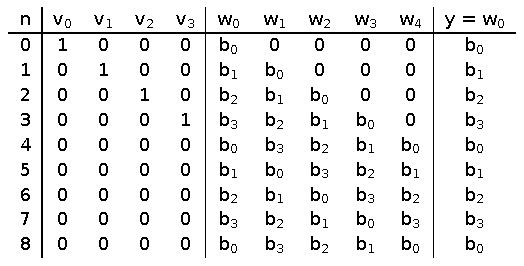
\includegraphics[width = \textwidth]{pic/TabelleDirektform.pdf}
		\end{minipage}

		\begin{minipage}{0.485\textwidth}
		\textbf{\textcolor{black}{\large{Implementierung mit kanonischer Form}}}\\[-0.2cm]
			\begin{itemize}
			 \item Zustände $w_i$ werden mit Null initialisiert.\\[-0.4cm]
			 \item FIR-Filter-Teil der periodisch angeregt wird, wodurch die $D$ Samples der Impulsantwort immer wieder generiert werden.\\[-0.4cm]
			 \item IIR-Filter-Teil der den Impuls $\delta(n)$ alle $D$ Samples wiederholt.\\[-0.1cm]
			\end{itemize}
			\hspace*{0.3cm}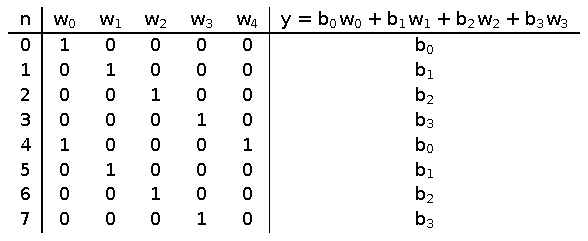
\includegraphics[width = \textwidth]{pic/TabelleKanonischeform.pdf}
		\end{minipage}\begin{minipage}{0.03\textwidth}$ $\end{minipage}
		\begin{minipage}{0.485\textwidth}
			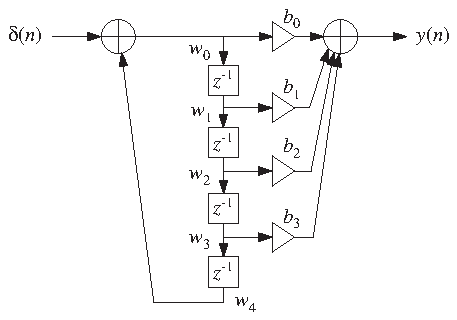
\includegraphics[width = 0.9\textwidth]{pic/periodischesWFGenKanonischeform.pdf}\\[0.1cm]
			\begin{tabular}{|lclll|}
			\hline &&&&$ $\\[-0.3cm]
			\multicolumn{5}{|l|}{$for\,\, n = 0,1,2,...\,\, do:$}\\
			&$w_0$&$ =$& $w_{D} + \delta(n)$&\\
			&$y$&$ = $&\multicolumn{2}{l|}{$b_0\,w_0 + b_1\,w_1 + b_2\,w_2 + ... + b_{D-1}\,w_{D-1}$}\\
			&$w_i$& $=$&$ w_{i-1}$ & $\qquad \quad i = D,D-1,\hdots,1$\\[0.1cm]
			\hline
			\end{tabular}
		\end{minipage}\\[0.1cm]
		
	\subsection{Spektrum periodischer Waveform Generatoren}
		\begin{itemize}
		 \item Da die Signalsequenzen $x(n)$ kausal (einseitig) sind, hat das Spektrum keine klaren Spektrallinien, sondern dominante Peaks bei der Grundfrequenz $f$ und dessen Harmonischen $mf$\\[0.2cm]
		 $H(\omega) = \dfrac{N(\omega)}{1-\e^{-j\omega D}} = \dfrac{N(\omega)}{2j\e^{j\omega D/2}\sin\left(\dfrac{\omega D}{2}\right)}\quad$\\[0.2cm]
		 $\Rightarrow\qquad$\fcolorbox{CadetRed}{white}{$\big|H(\omega)\big| = \dfrac{\big|N(\omega)\big|}{2\left|\sin\left(\dfrac{\omega D}{2}\right)\right|}$}$\quad$\fcolorbox{CadetRed}{white}{$\big|H(f)\big| = \dfrac{\big|N(f)\big|}{2\left|\sin\left(\dfrac{\pi fD}{f_s}\right)\right|}$}\\[-0.1cm]
		 \item Die Peaks kommen von den Polstellen von $|H(f)|$.\\[0.2cm]
		 $\sin\left(\dfrac{\pi fD}{f_s}\right) = 0\qquad\Rightarrow\quad\dfrac{\pi fD}{f_s}=m\pi$
		 $\qquad\Rightarrow\qquad$\fcolorbox{CadetRed}{white}{$f_m = m\dfrac{f_s}{D}\qquad\omega_m = \dfrac{2\pi m}{D}$}$\qquad m=0,1,...,D-1$
		 \\[0.3cm]
		 \begin{minipage}{0.75\textwidth}
			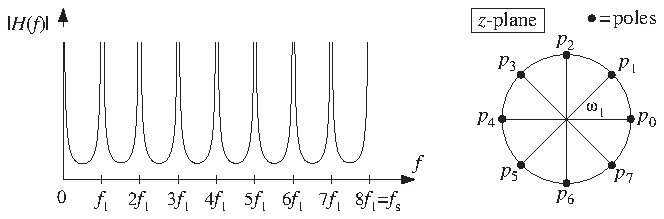
\includegraphics[width = \textwidth]{pic/SpektrumperiodischesDigitalesSignal.pdf}
		 \end{minipage}
		 \begin{minipage}{0.03\textwidth}$ $\end{minipage}
		 \begin{minipage}{0.27\textwidth}
			\fcolorbox{CadetRed}{white}{$z = p_m = \e^{j\omega_m}$}
		 \end{minipage}
		\end{itemize}
\newpage
\section{Wavetable Generatoren}
	\begin{itemize}
	 \item Statt zu filtern, können die $D$ Samples einer Periode auch in einer Tabelle abgespeichert werden und anschliessend immer wieder ''abgespielt'' werden.\\[-0.4cm]
	 \item Die Tabelle wird ein einem zirkularen Buffer $\bm{w} = [w_0,...,w_{D-1}]$ gespeichert und über einen Pointer $^*p = w[q]$, der rückwärts im Kreis wandert, ausgelesen.\\[-0.4cm]
	 \item Das Signal kann ganz einfach mit dem Startpunkt des Pointers $p$ verzögert werden:\\[0.1cm]
	 nicht verzögern:$\qquad$\fcolorbox{CadetRed}{white}{$p = \&w[0]$}$\qquad$um $m$-Samples verzögern:$\qquad$\fcolorbox{CadetRed}{white}{$p = \&w[m]$}\\[-0.4cm]
	 \item Der Buffer wird rückwärts gefüllt\\[0.15cm]
	 \fcolorbox{black}{white}{$\begin{array}{l}for\;i=0,1,...,D-1\;do:\\\quad w[(D-i)\%D] = b[i];\end{array}$}$\qquad$oder$\qquad$\fcolorbox{black}{white}{$\begin{array}{l}for\;i=0,1,...,D-1\;do:\\\quad w[i] = b[(D-i)\%D];\end{array}$}\\[-0.0cm]
	 \item Das Auslesen aus dem Buffer kann folgendermassen gemacht werden.\\[0.15cm]
	 \fcolorbox{black}{white}{$\begin{array}{l}q_0 = 0;\\ p = \& w[q_0];\\do\;\,forever:\\\quad y = *p;\\\quad q_{n+1} = (q_n-1)\%D;\\\quad p = \&w[q_{n+1}];\end{array}$}\\[-3.2cm]
	 \hspace*{4.6cm}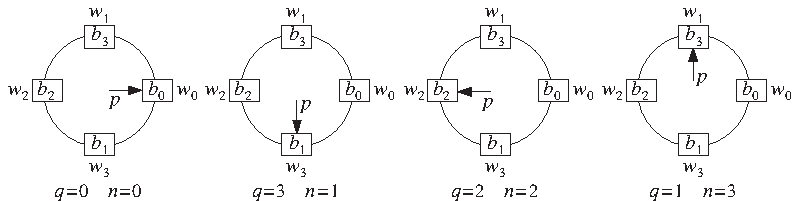
\includegraphics[width = 0.75\textwidth]{pic/wavetable4.pdf}\\[-0.2cm]
	\end{itemize}

	\subsection{Frequenz-Änderungen durch Wavetable-Manipulation}
		\begin{itemize}
		\item Die Abtastfrequenz $f_s$, die Länge der Wavetable $D$ und die Periode\\ $T_D$ bzw. die fundamentale Frequenz $f$ hängen folgendermassen\\ zusammen:\\[-1.1cm]
		\hspace*{12cm}\fcolorbox{CadetRed}{white}{$T_D = D\,T\qquad\Rightarrow\qquad f = \dfrac{f_s}{D}$}\\[-0.1cm]
		\item Die fundamentale Frequenz $f$ kann verändert werden,\\ indem die Länge der Wavetable $D$ verändert wird.\\[-1cm]
		\hspace*{10.6cm}\fcolorbox{CadetRed}{white}{$T_d = d\,T\qquad\Rightarrow\qquad f = \dfrac{f_s}{d}$}$\quad d\leq D$\\[-0.3cm]
		\item Wenn $D$ ein ganzzahliges Vielfaches von $d$ ist werden einfach Samples in der Wavetable übersprungen.\\
		\textbf{Beispiel:}\\ Nur jedes zweite Sample ausgeben$\quad\Rightarrow\quad$ fundamentale Frequenz $f$ verdoppeln.\\[-0.8cm]
		\hspace*{14.4cm}\fcolorbox{CadetRed}{white}{$c = \dfrac{D}{d}$}$\quad c\in\mathbb{Z}$\\[-0.1cm]
		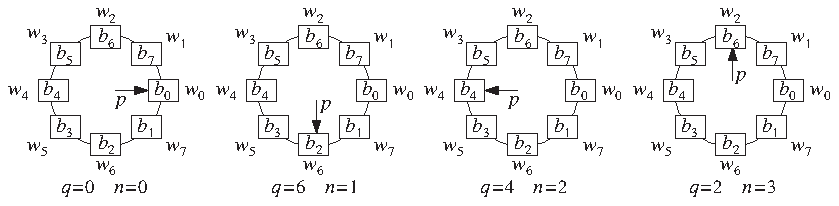
\includegraphics[width = 0.8\textwidth]{pic/wavetable6.pdf}\\[-0.6cm]
		\item Ist $D$ kein ganzzahliges Vielfaches von $d$ entstehen keine ganzzahligen Offsets und damit keine ganzzahligen Indizes $q_n$. Folglich müssen\\[-0.6cm]
		\begin{itemize}
		 \item Die Indizes aufgerundet, abgerundet oder normal gerundet werden.\\[-0.6cm]
		 \item Die Koeffizienten $b_i$ der Indizes davor und danach ($w\big[\lceil q_n\rceil\big],\,w\big[\lfloor q_n\rfloor\big]$) linear interpoliert werden. \\[-0.5cm]
		\end{itemize}
		\item Der Update des Indexes wird folgendermassen gemacht\\[0.1cm]
		\fcolorbox{CadetRed}{white}{$y(n)=\,\!^*p = w[q_n]$}$\qquad$\fcolorbox{CadetRed}{white}{$q_{n+1}=(q_n-c)\%D$}
		\end{itemize}
		\begin{danger}
		 \begin{tabularx}{\textwidth}{p{13cm}p{5cm}}
		  &\\[-0.8cm]
		  Damit das Abtasttheorem nicht verletzt wird muss $f$ innerhalb des Nyquist-Intervalls bleiben und für $c$ gilt damit: & $\begin{array}{l}\\[-0.1cm]\text{\fcolorbox{CadetRed}{white}{$-\dfrac{D}{2}\leq c \leq \dfrac{D}{2}$}}\end{array}$\\
		 \end{tabularx}
		\end{danger}	
